\documentclass[10pt,table]{beamer}
\usetheme[progressbar=frametitle]{metropolis}
\usepackage{appendixnumberbeamer}
\usepackage{booktabs}
\usepackage[scale=2]{ccicons}
\usepackage{xcolor}
\usepackage{pgfplots}
\usepgfplotslibrary{dateplot}

%\usepackage{xspace}
\newcommand{\themename}{\textbf{\textsc{metropolis}}\xspace}

\title{The SIR Model}
\subtitle{A Markov Chain model for disease spread}
\date{\today}
%\date{}
\author{Jackson Curtis}
\institute{Brigham Young University}
% \titlegraphic{\hfill\includegraphics[height=1.5cm]{logo.pdf}}

\begin{document}

\maketitle

\begin{frame}[fragile]{The Model}
The Susceptible-Infected-Recovered model describes how populations respond to disease.

$$\mathbf{E}\begin{bmatrix}
    p_{S,t}       \\
    p_{I,t}      \\

    p_{R,t}     
\end{bmatrix}
=
\begin{bmatrix}
a_{11} & 0 & 0 \\
a_{21} & a_{22} & 0 \\
0 & a_{32} & 1
\end{bmatrix}
\begin{bmatrix}
    p_{S,t-1}       \\
    p_{I,t-1}      \\

    p_{R,t-1}     
\end{bmatrix}
\label{sdf}
$$

The matrix in the middle is the transition matrix. The number in column i, row j is the probability of moving from state i to state j at each transition.
\end{frame}

\begin{frame}[fragile]{Boarding School Data}
\centering
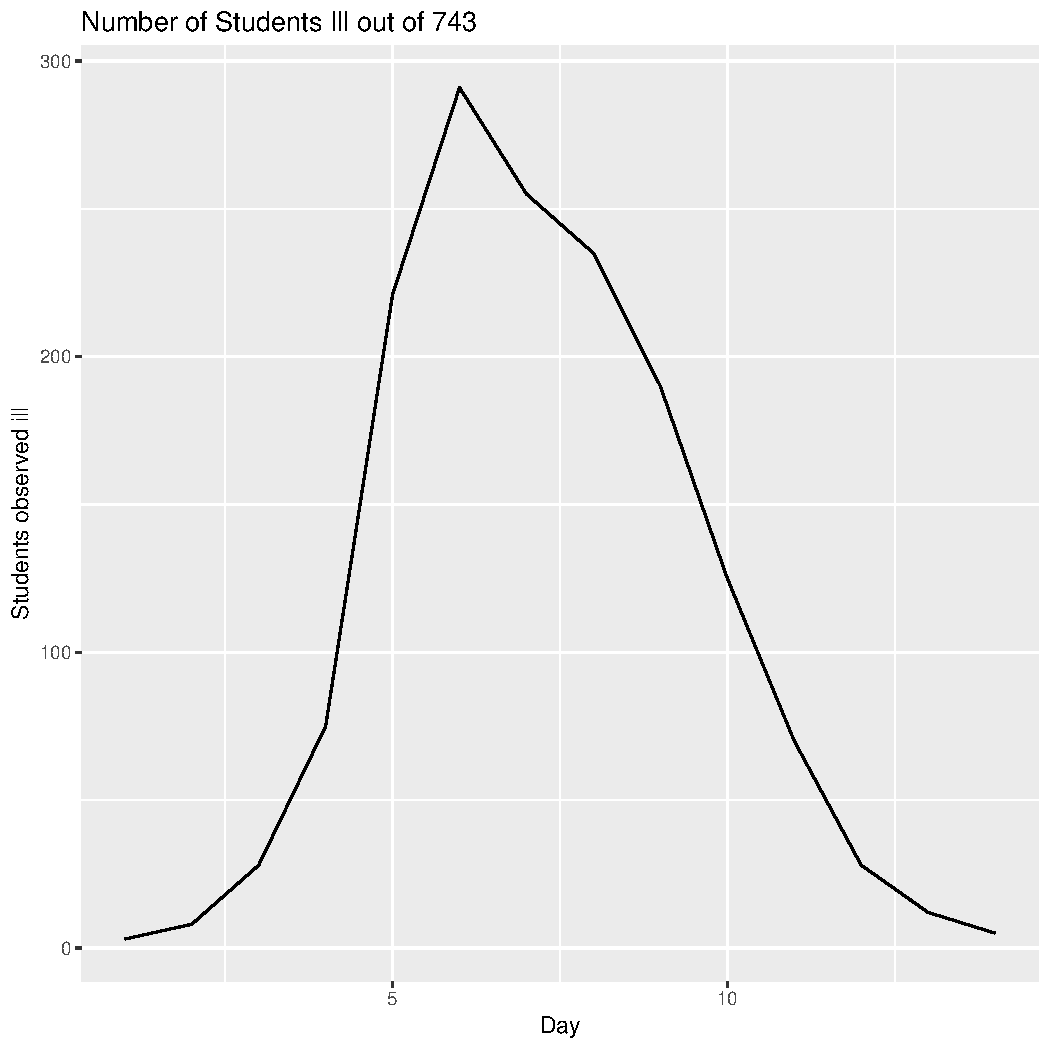
\includegraphics[scale=.45]{BoardingData.pdf}

\end{frame}

\begin{frame}{Deriving the Likelihood}
Our fourteen observations are not independent, so we can write the likelihood as: 
$$
f(x_1, x_2,...,x_n| a_{12}, a_{32}) = f(x_1| a_{12}, a_{32}) f(x_2|x_1, a_{12}, a_{32}) ... f(x_n|x_{n-1}, a_{12}, a_{32})
$$
\end{frame}

\begin{frame}{Deriving the Likelihood}
To address the fact that we didn't observe all states, we will sum over all possibilities. The R.V. $R_i$ will represent the number of people recovered on day i.
$$
f(x_i | x_{i-1}, a_{12}, a_{32}) =\sum_{j=0}^n f(x_i | x_{i-1}, a_{12}, a_{32}, R_i=j)\cdot Pr(R_i=j) 
\label{sum}
$$
\end{frame}


\begin{frame}{Deriving the Likelihood}
We will iteratively calculate $R_i$ as we move through the algorithm:

$$
Pr(R_i = r + h) = \sum_{j=0}^{x_{i-1}} Pr(H_i=j|R_{i-1}=r-j)\cdot Pr(R_{i-1}=r-j)
$$
\end{frame}

\begin{frame}{Deriving the Likelihood}
Now that we have R, we can calculate the probability of $x_i$ given $R_i$

\begin{multline*}
f(x_i|x_{i-1}, a_{12}, a_{32}, r) = \\ \sum_{h=0}^{x_{i-1}}       {{x_{i-1}}\choose{h}} a_{32}^h(1-a_{32})^{x_{i-1}-h}  {{n-x_{i-1}-r}\choose{x_i-(x_{i-1}-h)}}  a_{12}^{x_i-(x_{i-1}-h)} (1-a_{12})^{n - r - x_i-h}I(x)  \end{multline*} $$
\text{where } I(x) = \begin{cases} 1 & \text{for } x_{i-1}-h\leq x_i\leq n-r  \\ 0 &\text{otherwise} \end{cases}$$


\end{frame}
\begin{frame}{Maximizing the Likelihood}
The resulting likelihood involves a triple summation over time periods, possible values of R, and possible values of H (people healed), and two binomial densities. Needless to say, I didn't calculate the Hessian. 
\begin{itemize}
\item Nelder-Mead constrained optimization (constraining both parameters between 0 and 1)
\item Coded likelihood in C++ for faster evaluation
\end{itemize}

\end{frame}

\begin{frame}{So...Did it work?}
500 Simulations of each scenario
\begin{table}
\centering
\setlength{\tabcolsep}{5pt}

\begin{tabular}{|c|c|c|c|c|c|}
\hline
Pop. & No obs. & $a_{12}$ & $a_{32}$ & 95\% CI on $\hat{a}_{12}$ & 95\% CI on $\hat{a}_{32}$  \\ \hline 
743 & 14 & 0.0848 & 0.3420 &\cellcolor{green!25}(0.0845, 0.0857) & \cellcolor{green!25}(0.341, 0.345) \\ \hline
500 & 14 & 0.02 &0.3 & \cellcolor{red!25} (0.020, 0.021) &\cellcolor{red!25}  (0.305, 0.319)\\ \hline
473 & 14 & 0.0848 & 0.3420 &\cellcolor{green!25} (0.084, 0.086) & \cellcolor{green!25}(0.340, 0.345) \\ \hline
200 & 6 & 0.1 &.3 &\cellcolor{red!25} (0.101, 0.104)&\cellcolor{red!25}  (0.301, 0.314)\\ \hline 
100 & 14 & 0.2 & 0.7 &\cellcolor{red!25} (0.202, 0.206) & \cellcolor{green!25}(0.700, 0.708) \\ \hline
100 & 14 & 0.7 & 0.2 &\cellcolor{green!25}(0.700, 0.707) & \cellcolor{red!25} (0.222, 0.225)\\ \hline
100 & 14 &0.5 &0.5 &\cellcolor{red!25} (0.505, 0.513) &\cellcolor{red!25} (0.534, 0.537)\\ \hline

50 & 20 & 0.1 &0.3 &\cellcolor{green!25}(0.099, 0.104) & \cellcolor{red!25} (0.282, 0.291)\\ \hline

20 & 8 & 0.4 & 0.3 & \cellcolor{red!25} (0.405, 0.422) & \cellcolor{red!25} (0.304, 0.315)\\ \hline



\end{tabular}
\label{tab1}
\end{table}

\end{frame}

\begin{frame}{Lack of Fit}
\begin{figure}
\centering
\begin{minipage}{.4\textwidth}
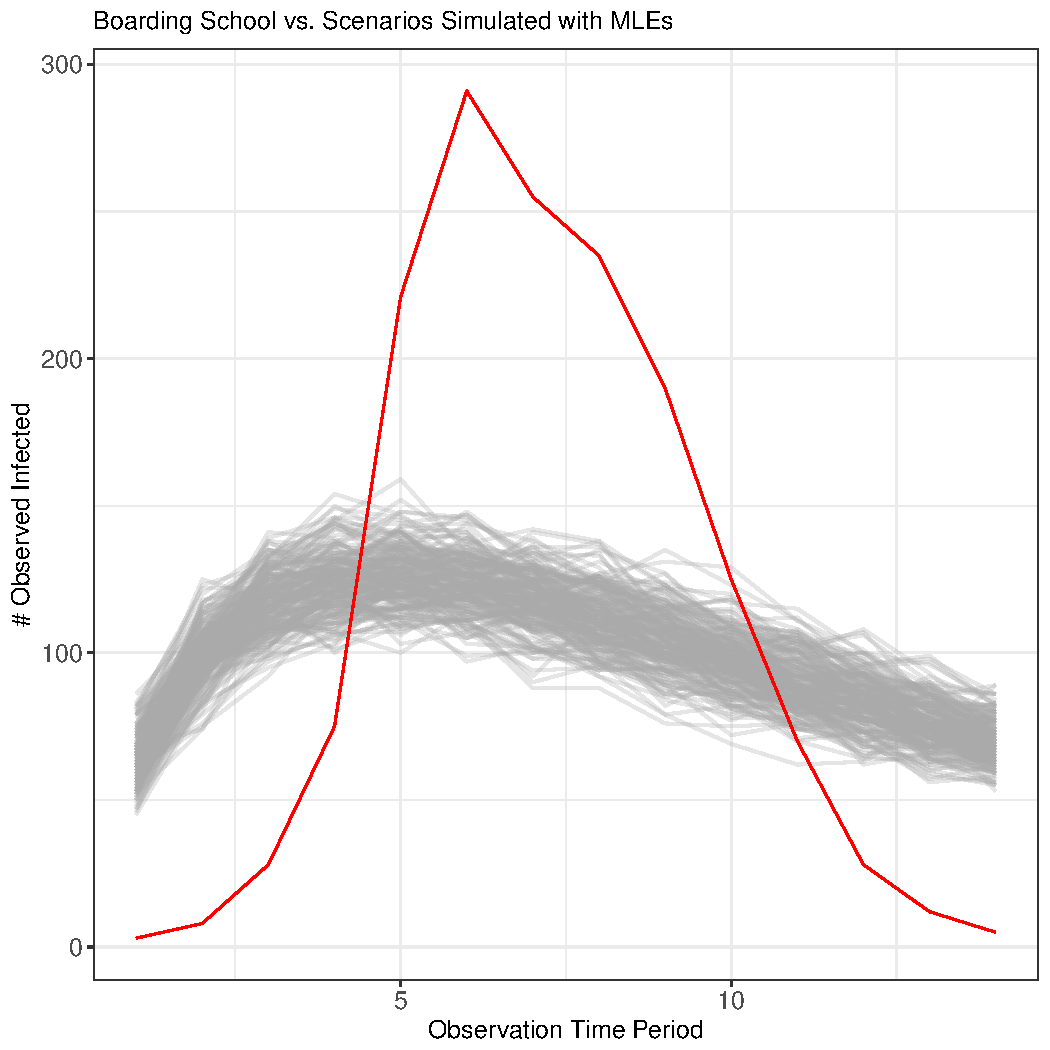
\includegraphics[width=1\linewidth]{LackOfFit.pdf}
\end{minipage}%
\begin{minipage}{.4\textwidth}

\centering
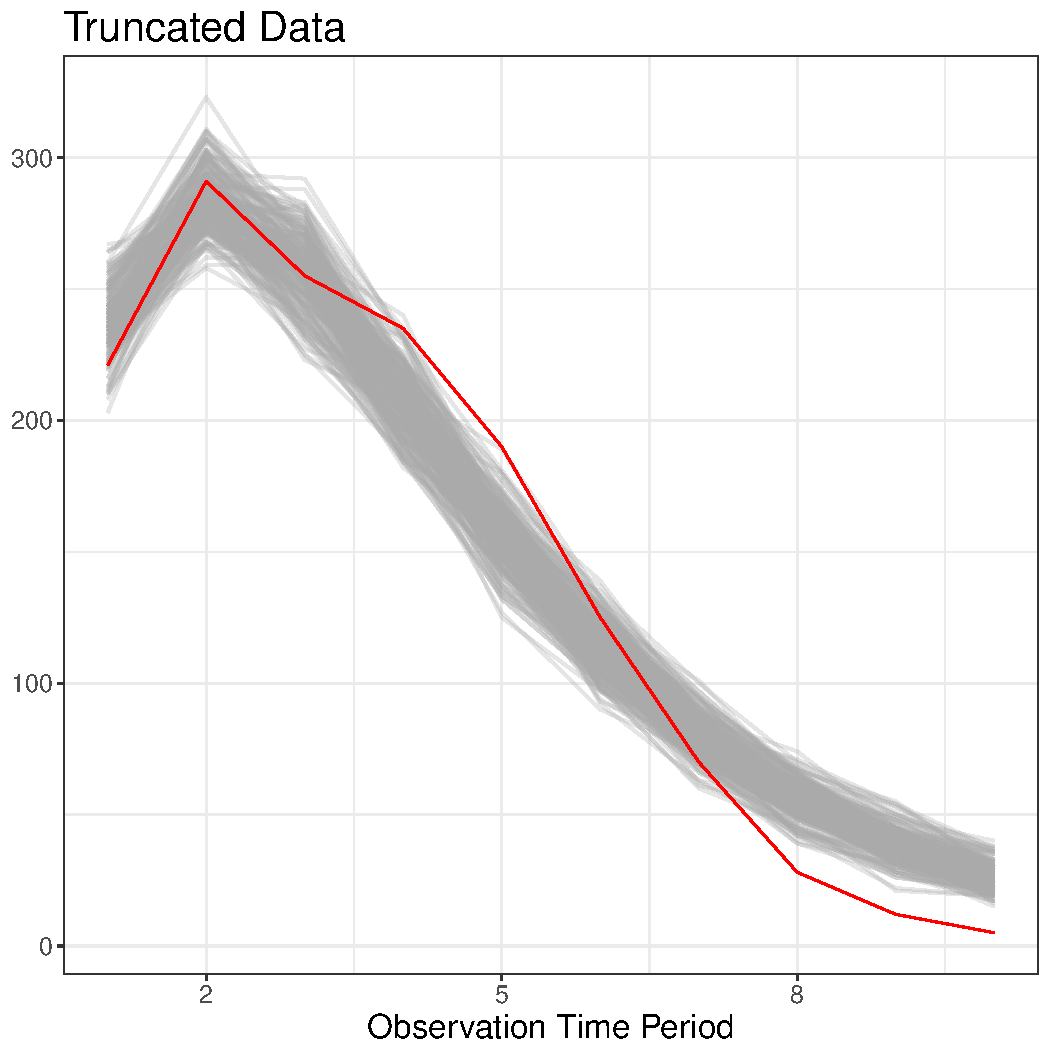
\includegraphics[width=1\linewidth]{BetterFit.pdf}
\end{minipage}
\caption{Actual data vs. 200 simulations using MLE as parameters for full dataset and dataset without first four days}
\label{plot1}
\end{figure}

\end{frame}

\begin{frame}{Inference}
\centering
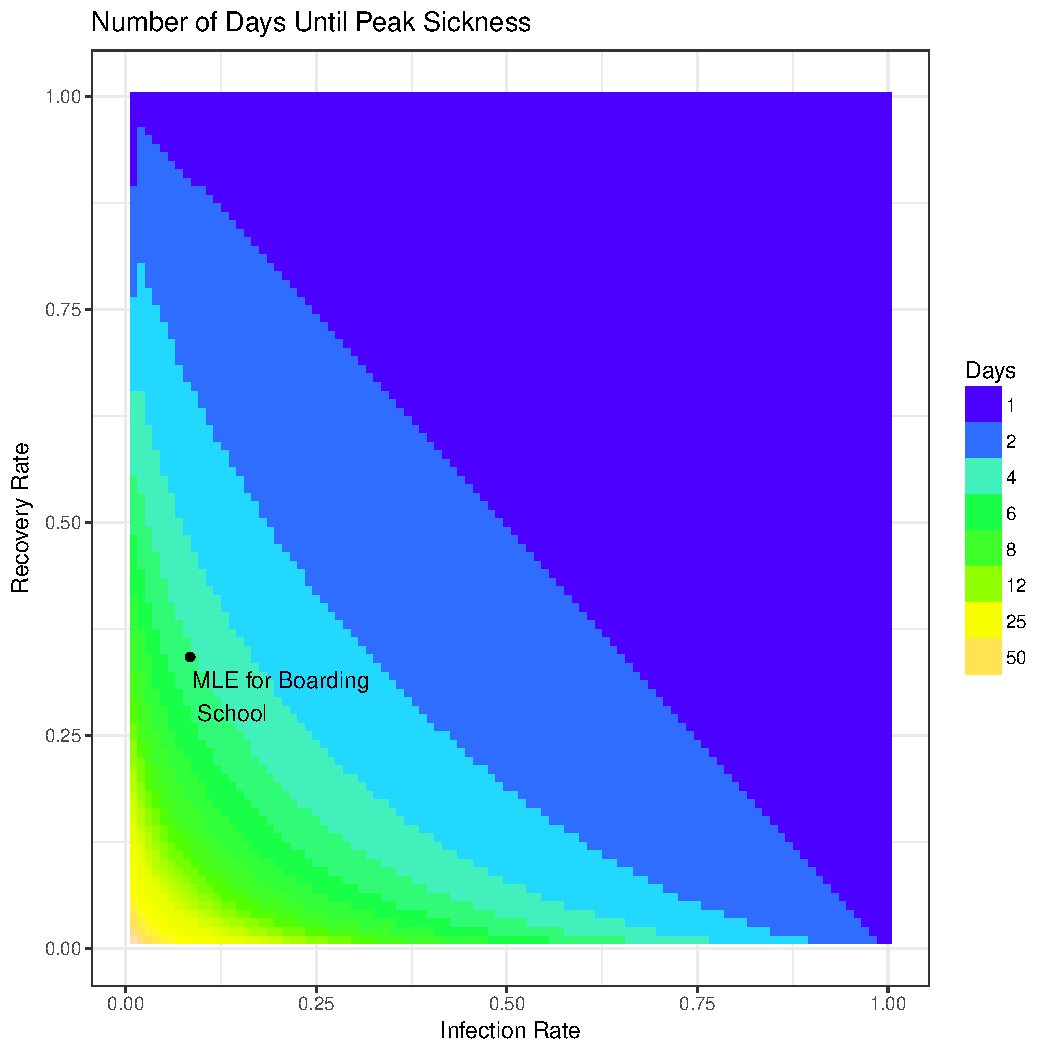
\includegraphics[scale=.45]{DayGrid.pdf}
\end{frame}

\begin{frame}{Inference}
\centering
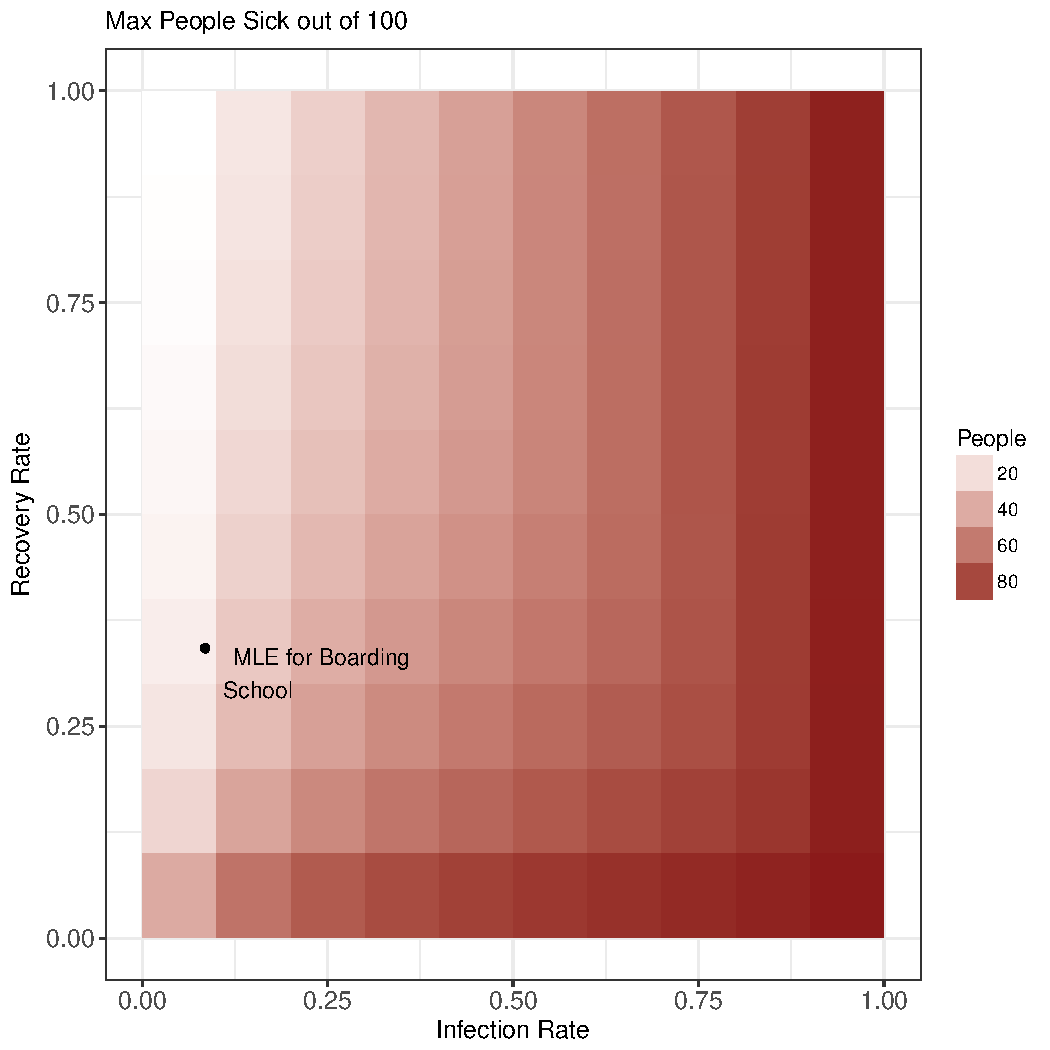
\includegraphics[scale=.45]{MaxGrid.pdf}
\end{frame}
\begin{frame}{}
The end
\end{frame}


\end{document}

Beamer theme created by Matthias Vogelgesang 
More information found at https://github.com/matze/mtheme